%definira klasu dokumenta 
\documentclass[12pt]{report} 

%prostor izmedu naredbi \documentclass i \begin{document} se zove uvod. U njemu se nalaze naredbe koje se odnose na cijeli dokument

%osnovni LaTex ne može riješiti sve probleme, pa se koriste različiti paketi koji olakšavaju izradu željenog dokumenta
\usepackage[croatian]{babel} 
\usepackage{amssymb}
\usepackage{amsmath}
\usepackage{txfonts}
\usepackage{mathdots}
\usepackage{titlesec}
\usepackage{array}
\usepackage{lastpage}
\usepackage{etoolbox}
\usepackage{tabularray}
\usepackage{color, colortbl}
\usepackage{adjustbox}
\usepackage{geometry}
\usepackage[classicReIm]{kpfonts}
\usepackage{hyperref}
\usepackage{fancyhdr}
\usepackage{graphicx}

\usepackage{float}
\usepackage{setspace}
\restylefloat{table}


\patchcmd{\chapter}{\thispagestyle{plain}}{\thispagestyle{fancy}}{}{} %redefiniranje stila stranice u paketu fancyhdr

%oblik naslova poglavlja
\titleformat{\chapter}{\normalfont\huge\bfseries}{\thechapter.}{20pt}{\Huge}
\titlespacing{\chapter}{0pt}{0pt}{40pt}


\linespread{1.3} %razmak između redaka

\geometry{a4paper, left=1in, top=1in,}  %oblik stranice

\hypersetup{ colorlinks, citecolor=black, filecolor=black, linkcolor=black,	urlcolor=black }   %izgled poveznice


%prored smanjen između redaka u nabrajanjima i popisima
\newenvironment{packed_enum}{
	\begin{enumerate}
		\setlength{\itemsep}{0pt}
		\setlength{\parskip}{0pt}
		\setlength{\parsep}{0pt}
	}{\end{enumerate}}

\newenvironment{packed_item}{
	\begin{itemize}
		\setlength{\itemsep}{0pt}
		\setlength{\parskip}{0pt}
		\setlength{\parsep}{0pt}
	}{\end{itemize}}




%boja za privatni i udaljeni kljuc u tablicama
\definecolor{LightBlue}{rgb}{0.9,0.9,1}
\definecolor{LightGreen}{rgb}{0.9,1,0.9}

%Promjena teksta za dugačke tablice
\DefTblrTemplate{contfoot-text}{normal}{Nastavljeno na idućoj stranici}
\SetTblrTemplate{contfoot-text}{normal}
\DefTblrTemplate{conthead-text}{normal}{(Nastavljeno)}
\SetTblrTemplate{conthead-text}{normal}
\DefTblrTemplate{middlehead,lasthead}{normal}{Nastavljeno od prethodne stranice}
\SetTblrTemplate{middlehead,lasthead}{normal}

%podesavanje zaglavlja i podnožja

\pagestyle{fancy}
\lhead{Programsko inženjerstvo}
\rhead{CookBooked}
\lfoot{ErrorMasters}
\cfoot{stranica \thepage/\pageref{LastPage}}
\rfoot{\today}
\renewcommand{\headrulewidth}{0.2pt}
\renewcommand{\footrulewidth}{0.2pt}


\begin{document} 
	
	
	
	\begin{titlepage}
		\begin{center}
			\vspace*{\stretch{1.0}} %u kombinaciji s ostalim \vspace naredbama definira razmak između redaka teksta
			\LARGE Programsko inženjerstvo\\
			\large Ak. god. 2023./2024.\\
			
			\vspace*{\stretch{3.0}}
			
			\huge CookBooked\\
			\Large Dokumentacija, Rev. \textit{1}\\
			
			\vspace*{\stretch{12.0}}
			\normalsize
			Grupa: \textit{ErrorMasters}\\
			Voditelj: \textit{Matija Alojz Stuhne}\\
			
			
			\vspace*{\stretch{1.0}}
			Datum predaje: \textit{16. 11. 2023.}\\
	
			\vspace*{\stretch{4.0}}
			
			Nastavnik: \textit{Nikolina Frid}\\
		
		\end{center}

	
	\end{titlepage}

	
	\tableofcontents


	\chapter{Dnevnik promjena dokumentacije}
				
		
		\begin{longtblr}[
				label=none
			]{
				width = \textwidth, 
				colspec={|X[2]|X[13]|X[3]|X[3]|}, 
				rowhead = 1
			}
			\hline
			\textbf{Rev.}	& \textbf{Opis promjene/dodatka} & \textbf{Autori} & \textbf{Datum}\\[3pt] \hline
			0.1 & Napravljen predložak.	& Matija Alojz Stuhne & 23.10.2023. 		\\[3pt] \hline
			0.1.1 & Osvježen predložak s podatcima grupe. & Matija Alojz Stuhne & 30.10.2023. \\[3pt] \hline 
			0.2	& Dodan opis projektnog zadatka. & Matija Alojz Stuhne & 30.10.2023. 	\\[3pt] \hline 
			0.3 & Dodani dionici, aktori i njihovi funkcionalni zahtjevi & Matija Alojz Stuhne & 31.10.2023. \\[3pt] \hline 
			0.4 & Dodani obrasci uporabe & Matija Alojz Stuhne & 31.10.2023. \\[3pt] \hline 
			0.4.1 & Manje promjene dokumentacije & Matija Alojz Stuhne & 01.11.2023. \\[3pt] \hline 
			0.5 & Dodani dijagrami obrazaca uporabe & Marko Dananić & 03.11.2023. \\[3pt] \hline 
			0.5.1 & Dodani dijagrami obrazaca uporabe (u dokument)\newline Manje promjene dokumentacije & Matija Alojz Stuhne & 03.11.2023. \\[3pt] \hline 
			0.5.2 & Manje promjene dijagrama obrazaca uporabe & Marko Dananić, Matija Alojz Stuhne & 04.11.2023 \\[3pt] \hline 
			0.6 & Dodani sekvencijski dijagrami & Matija Alojz Stuhne & 04.11.2023. \\[3pt] \hline
			0.6.1 & Dodani opisi sekvencijskih dijagrama \newline \textit{Pushed by M. A. Stuhne}& Marko Dananić & 07.11.2023. \\[3pt] \hline  
			0.6.2 & Manje promjene sekvencijskih dijagrama& Matija Alojz Stuhne & 15.11.2023. \\[3pt] \hline
			0.6.3 & Manje promjene dokumentacije - sastanci, dnevnik promjena& Matija Alojz Stuhne & 15.11.2023. \\[3pt] \hline
			0.7 & Dodani prikazi relacija baze podataka & Matija Alojz Stuhne & 15.11.2023. \\[3pt] \hline
			0.7.1 & Dodani opisi prikaza relacija baze podataka & Matija Alojz Stuhne & 16.11.2023. \\[3pt] \hline
			0.8. & Dodani dijagrami razreda \newline \textit{Pushed by M. A. Stuhne}& Marko Dananić, Petra Habjanec & 16.11.2023. \\[3pt] \hline  
			0.8.1 & Dodani ostali zahtjevi sustava & Matija Alojz Stuhne & 16.11.2023. \\[3pt] \hline  
			0.8.2 & Manje promjene dijagrama obrazaca uporabe \newline \textit{Pushed by M. A. Stuhne}& Marko Dananić & 16.11.2023. \\[3pt] \hline  
			0.8.3 & Dodan uvodni tekst za dijagrame razreda & Matija Alojz Stuhne & 16.11.2023. \\[3pt] \hline  
			\textbf{1.0.0} & Korigiranje teksta i provjera dokumentacije & Matija Alojz Stuhne & 16.11.2023. \\[3pt] \hline
			1.1.0 & Započeta razrada 5. poglavlja & Matija Alojz Stuhne & 2.1.2024. \\[3pt] \hline  
		\end{longtblr}

	\chapter{Opis projektnog zadatka}
		
		\textbf{\textit{dio 1. revizije}}\\
		
		Cilj ovog projekta je razviti programsku podršku za stvaranje web aplikacije "CookBooked" koja će
		omogućiti korisnicima razmjenu recepata za kuhanje i pečenje kolača te povezivanje i komunikaciju s autorima
		recepata. Platforma će ponuditi različit spektar mogućnosti ovisno o tome je li korisnik registriran ili nije.

		Prilikom pokretanja sustava prikazuje se izbornik recepata po kategorijama (prigoda, namirnice, zemlja podrijetla recepta).		
		
		Neregistrirani korisnici mogu \textbf{samo pregledavati} recepte temeljem kategorija.
		Neregistrirani korisnici vide sve detalje recepata (naslov, sastojci, koraci pripreme, posebne oznake...).
		Kako bi korisniku bilo omogućeno vršiti dodatne radnje (objava recepata, komentiranje recepata, spremanje recepata...),
		potrebno se prijaviti sa postojećim korisničkim računom ili registracijom kreirati novi korisnički račun.

		\textbf{
			Za kreiranje novog korisničkog računa potrebni su slijedeći podatci:
		}
		\begin{packed_item}
			\item \textit{korisničko ime}
			\item \textit{lozinka}
			\item \textit{ime}
			\item \textit{prezime}
			\item \textit{broj mobitela}
			\item \textit{email adresa}
		\end{packed_item}

		Registracijom u sustav korisniku se dodjeljuju prava klijenta, a naknadno mu se mogu dodijeliti prava
		vlasnika portala ili administratora. Registrirani korisnik može objavljivati recepte za kuhanje i pečenje,
		komentirati na ostale recepte itd.
				
		\underline{\textit{Klijent}} objavom recepta postaje njegov autor. Autori recepata mogu komunicirati s ostalim
		korisnicima vezano za svoje recepte (termin komunikacija = chat, videopozivi itd.). Klijent ima mogućnost označavanja, 
		komentiranja i spremanja recepata za buduću referencu. Također, kao dodatna mogućnost, pruža se i opcija praćenja 
		omiljenih autora (obavijesti). Klijent ima dvije vrste profila, javni i privatni. Na javnom su prikazani recepti,
		pratitelji i autori koje klijent prati; dok su na privatnom prikazane osobne informacije kojima klijent može
		upravljati (korisničko ime, lozinka, e-mail adresa, ime, prezime...).
		
		\underline{\textit{Vlasnik}} portala ima dodatne mogućnosti brisanja neželjenih recepata i/ili komentara ispod njih
		te mogućnost brisanja i/ili dodavanja novih kategorija recepata.

		\underline{\textit{Administrator}} sustava ima najveće ovlasti. On ima pristup bazi s popisom registriranih korisnika
		te ima mogućnost brisanja ili promijene korisničkih podataka. Također, ima svu funkcionalnost vlasnika restorana.
		
		\bigskip

		\textbf{Postojeća slična rješenja:}

		\url{https://www.coolinarika.com/}

		\begin{figure}[H]
			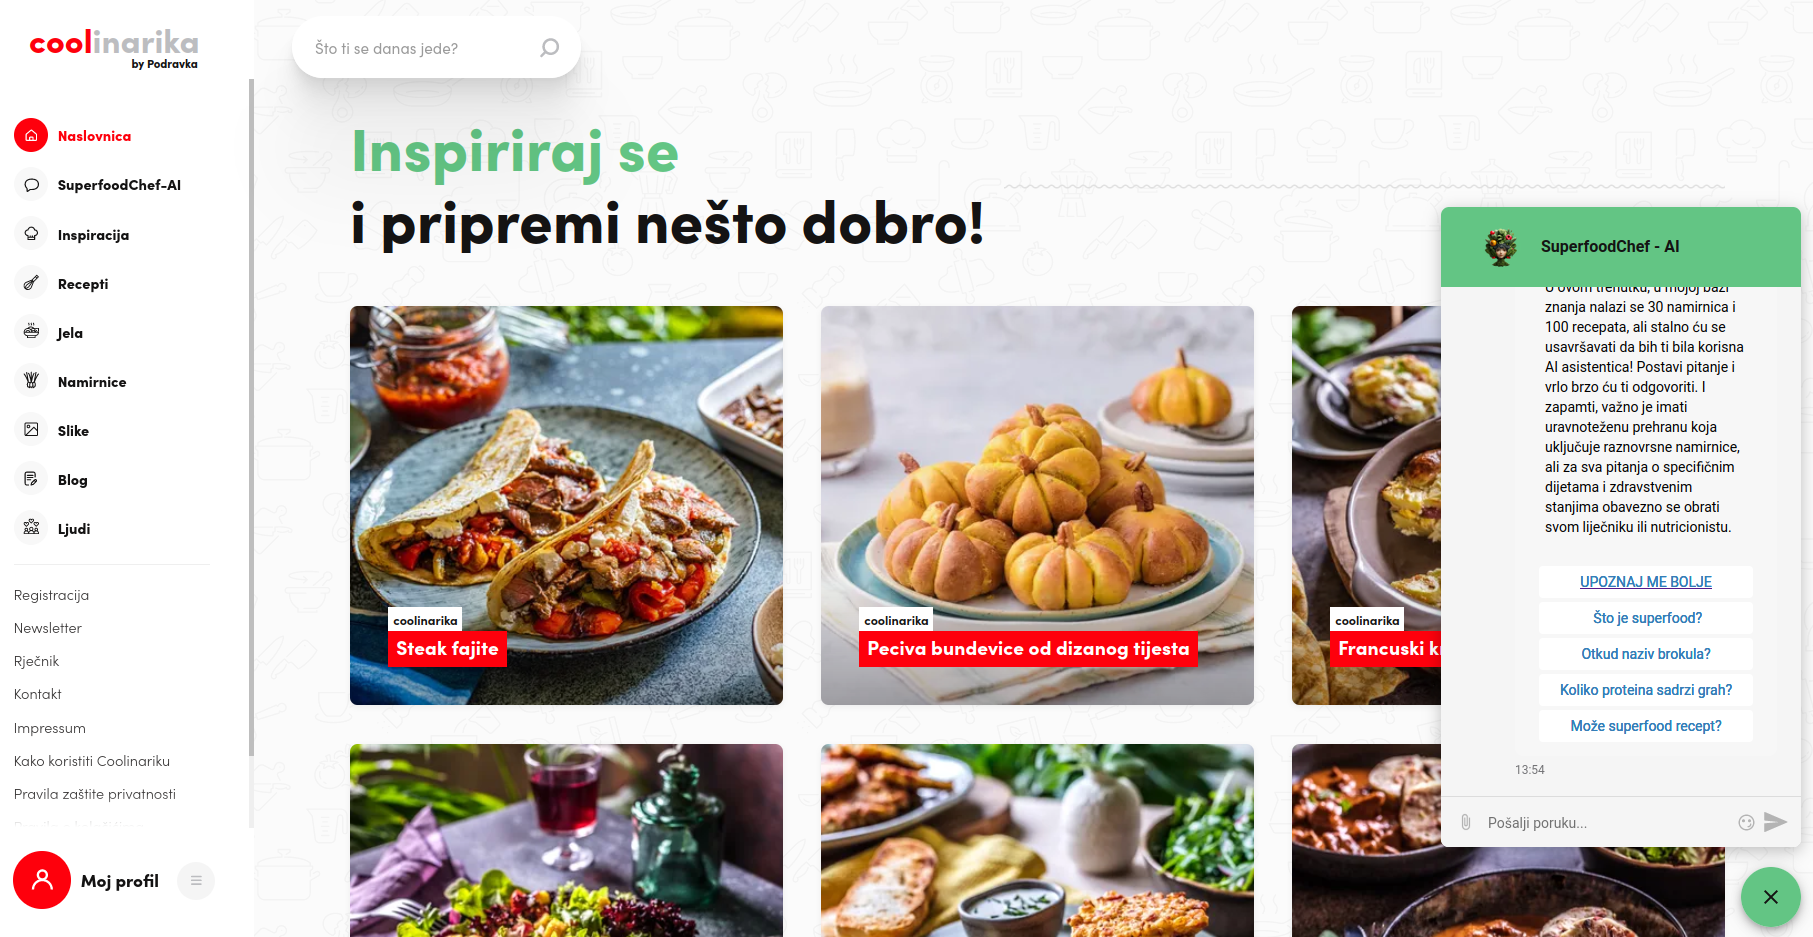
\includegraphics[scale=0.2]{slike/coolinarika.png}
			\centering
			\caption{Izgled coolinarika web portala}
			\label{fig:coolinarika}
		\end{figure}

		\url{https://recepti.index.hr/}

		\begin{figure}[H]
			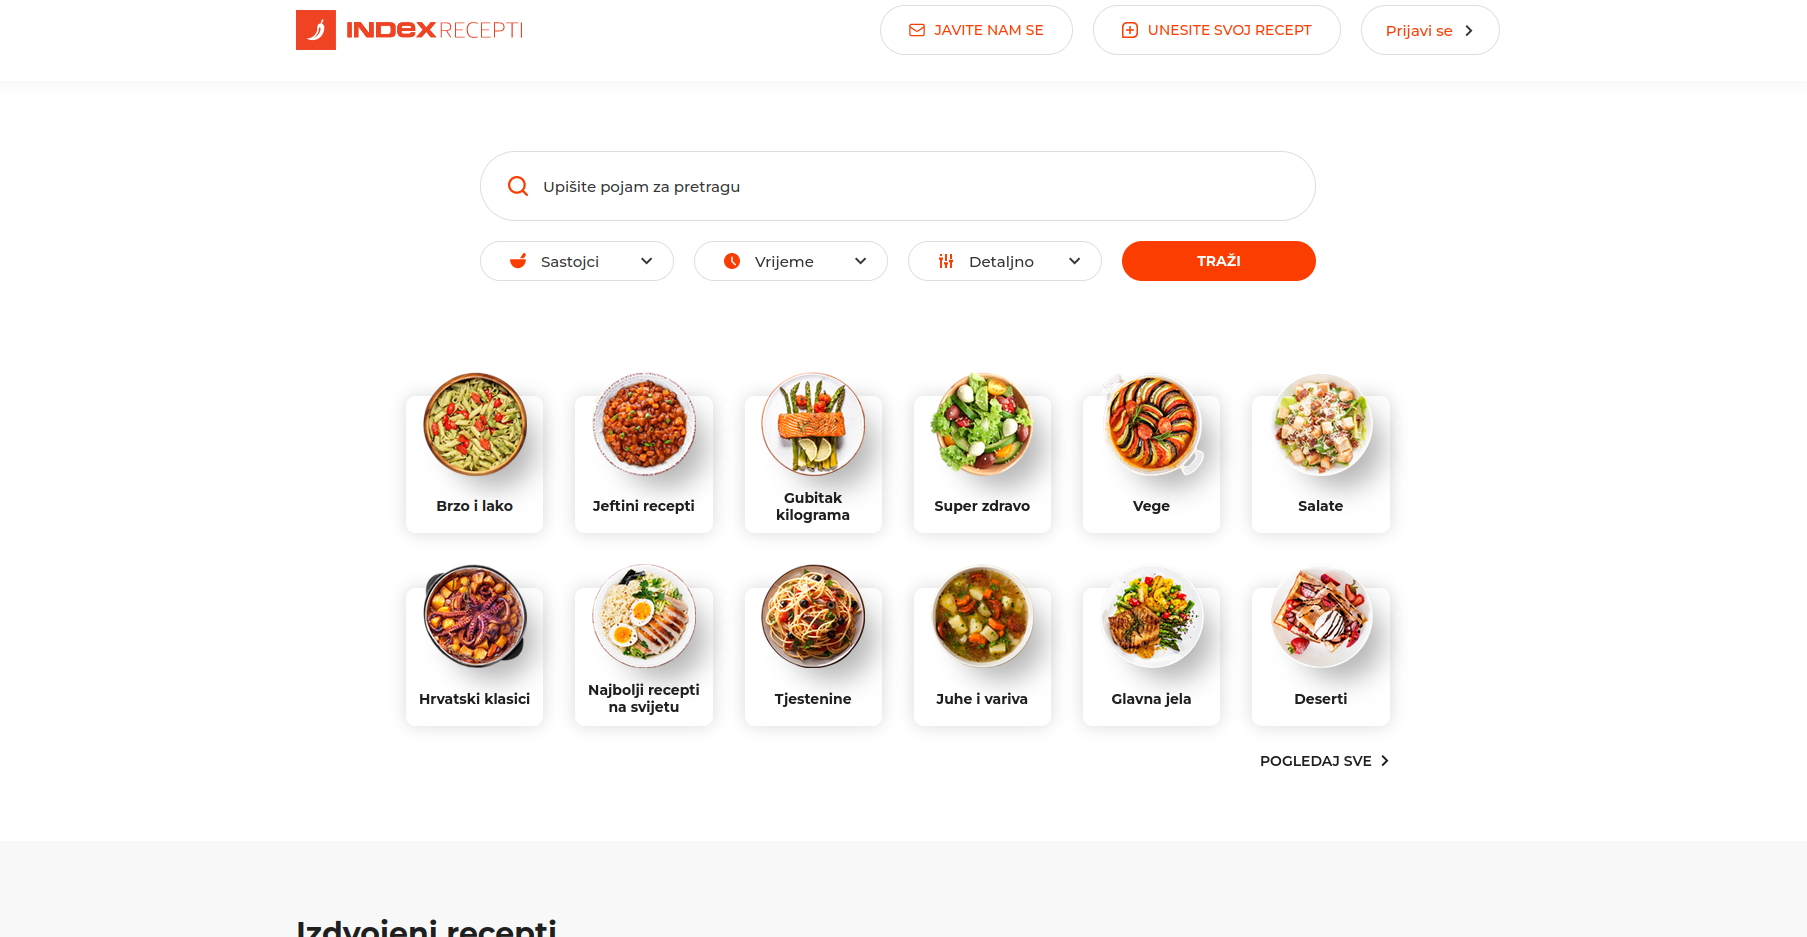
\includegraphics[scale=0.2]{slike/index-recepti.png} 
			\centering
			\caption{Izgled index-recepti web portala}
			\label{fig:index-recepti}
		\end{figure}

		\bigskip
		\bigskip
		\bigskip

		Postojeća rješenja baziraju se na proširenoj funkcionalnosti (osim kolača nude i recepte ostalih jela).
		Coolinarika nudi i dodatnu funckionalost razgovora sa AI ChatBot-om koji pomaže ljudima oko generalnog
		pojma prehrane. Također, Coolinarika ima i blog te pregled svojstava namirnica koje se koriste u receptima.

		\bigskip

		\textbf{Mogućnost nadogradnje web portala CookBooked:}

		Web portal CookBooked primarno je zamišljen kao pomoćnik u kuhanju i pečenju kolača.
		Kao takav, usmjeren je na korisnike čiji je primarni interes područje slastica.

		\smallskip

		Svaka nadogradnja postojećeg portala morala bi biti dobro iskomunicirana sa postojećim klijentima.

		\smallskip

		Mogućnosti nadogradnje:
		
		\begin{packed_item}
			\item \textit{dodavanje recepata koji nisu vezani za kolače}
			\item \textit{prijenos uživo pripremanja recepata}
			\item \textit{dodavanje oglasnik poslova vezanih uz kulinarstvo/slastičarstvo}
			\item \textit{dodavanje premium sadržaja dostupnog samo plaćenim klijentima}
		\end{packed_item}

		\textbf{Financiranje web portala CookBooked:}

		Održavanje i nadogradnja web portala CookBooked planiraju se financirati iz slijedećih izvora:

		\begin{packed_item}
			\item \textit{plaćeni oglasi na web portalu}
			\item \textit{prodaja premium korisničkih mogućnosti (u planu)}
			\item \textit{donacije}
		\end{packed_item}




		\eject
		
	
	\chapter{Specifikacija programske potpore}
		
	\section{Funkcionalni zahtjevi}
			
			\textbf{\textit{dio 1. revizije}}\\
			
			\textit{Navesti \textbf{dionike} koji imaju \textbf{interes u ovom sustavu} ili  \textbf{su nositelji odgovornosti}. To su prije svega korisnici, ali i administratori sustava, naručitelji, razvojni tim.}\\
				
			\textit{Navesti \textbf{aktore} koji izravno \textbf{koriste} ili \textbf{komuniciraju sa sustavom}. Oni mogu imati inicijatorsku ulogu, tj. započinju određene procese u sustavu ili samo sudioničku ulogu, tj. obavljaju određeni posao. Za svakog aktora navesti funkcionalne zahtjeve koji se na njega odnose.}\\
			
			
			\noindent \textbf{Dionici:}
			
			\begin{packed_enum}
				
				\item Dionik 1
				\item Dionik 2				
				\item ...
				
			\end{packed_enum}
			
			\noindent \textbf{Aktori i njihovi funkcionalni zahtjevi:}
			
			
			\begin{packed_enum}
				\item  \underbar{Aktor 1 (inicijator) može:}
				
				\begin{packed_enum}
					
					\item funkcionalnost 1
					\item funkcionalnost 2
					\begin{packed_enum}
						
						\item  podfunkcionalnost 1 
						\item  podfunkcionalnost 2
				
					\end{packed_enum}
					\item  funkcionalnost 3
					
				\end{packed_enum}
			
				\item  \underbar{Aktor 2 (sudionik) može:}
				
				\begin{packed_enum}
					
					\item funkcionalnost 1
					\item funkcionalnost 2
					
				\end{packed_enum}
			\end{packed_enum}
			
			\eject 
			
			
				
			\subsection{Obrasci uporabe}
				
				\textbf{\textit{dio 1. revizije}}
				
				\subsubsection{Opis obrazaca uporabe}
					\textit{Funkcionalne zahtjeve razraditi u obliku obrazaca uporabe. Svaki obrazac je potrebno razraditi prema donjem predlošku. Ukoliko u nekom koraku može doći do odstupanja, potrebno je to odstupanje opisati i po mogućnosti ponuditi rješenje kojim bi se tijek obrasca vratio na osnovni tijek.}\\
					

					\noindent \underbar{\textbf{UC$<$broj obrasca$>$ -$<$ime obrasca$>$}}
					\begin{packed_item}
	
						\item \textbf{Glavni sudionik: }$<$sudionik$>$
						\item  \textbf{Cilj:} $<$cilj$>$
						\item  \textbf{Sudionici:} $<$sudionici$>$
						\item  \textbf{Preduvjet:} $<$preduvjet$>$
						\item  \textbf{Opis osnovnog tijeka:}
						
						\item[] \begin{packed_enum}
	
							\item $<$opis korak jedan$>$
							\item $<$opis korak dva$>$
							\item $<$opis korak tri$>$
							\item $<$opis korak četiri$>$
							\item $<$opis korak pet$>$
						\end{packed_enum}
						
						\item  \textbf{Opis mogućih odstupanja:}
						
						\item[] \begin{packed_item}
	
							\item[2.a] $<$opis mogućeg scenarija odstupanja u koraku 2$>$
							\item[] \begin{packed_enum}
								
								\item $<$opis rješenja mogućeg scenarija korak 1$>$
								\item $<$opis rješenja mogućeg scenarija korak 2$>$
								
							\end{packed_enum}
							\item[2.b] $<$opis mogućeg scenarija odstupanja u koraku 2$>$
							\item[3.a] $<$opis mogućeg scenarija odstupanja  u koraku 3$>$
							
						\end{packed_item}
					\end{packed_item}
				
					
				\subsubsection{Dijagrami obrazaca uporabe}
					
					\textit{Prikazati odnos aktora i obrazaca uporabe odgovarajućim UML dijagramom. Nije nužno nacrtati sve na jednom dijagramu. Modelirati po razinama apstrakcije i skupovima srodnih funkcionalnosti.}
				\eject		
				
			\subsection{Sekvencijski dijagrami}
				
				\textbf{\textit{dio 1. revizije}}\\
				
				\textit{Nacrtati sekvencijske dijagrame koji modeliraju najvažnije dijelove sustava (max. 4 dijagrama). Ukoliko postoji nedoumica oko odabira, razjasniti s asistentom. Uz svaki dijagram napisati detaljni opis dijagrama.}
				\eject
	
		\section{Ostali zahtjevi}
		
			\textbf{\textit{dio 1. revizije}}\\
		 
			 \textit{Nefunkcionalni zahtjevi i zahtjevi domene primjene dopunjuju funkcionalne zahtjeve. Oni opisuju \textbf{kako se sustav treba ponašati} i koja \textbf{ograničenja} treba poštivati (performanse, korisničko iskustvo, pouzdanost, standardi kvalitete, sigurnost...). Primjeri takvih zahtjeva u Vašem projektu mogu biti: podržani jezici korisničkog sučelja, vrijeme odziva, najveći mogući podržani broj korisnika, podržane web/mobilne platforme, razina zaštite (protokoli komunikacije, kriptiranje...)... Svaki takav zahtjev potrebno je navesti u jednoj ili dvije rečenice.}
			 
			 
			 
	
	\chapter{Arhitektura i dizajn sustava}

		Arhitektura se može podijeliti na tri podsustava:
		\begin{itemize}
			\item 	Web poslužitelj
			\item 	Web aplikacija
			\item 	Baza podataka		
		\end{itemize}

		\underbar{Web preglednik} predstavlja softverski program koji omogućuje korisnicima 
		pregledavanje web-stranica i konzumiranje povezanih multimedijskih sadržaja. 
		Svaki internetski preglednik djeluje kao prevoditelj, interpretirajući kôd web 
		stranica napisan u određenom programskom jeziku i pretvarajući ga u vizualni 
		format razumljiv svakom korisniku. Drugim riječima, stranice su izvorno napisane 
		u kodu, a \textit{web preglednik} ih interpretira kako bi korisnicima pružio čitljiv i 
		interaktivan prikaz. Kada korisnik želi pristupiti određenoj web stranici, 
		šalje zahtjev \textit{web poslužitelju} putem \textit{web preglednika}, što pokreće proces 
		prijenosa informacija i omogućava korisnicima interakciju s odabranim sadržajem.


		\underbar{Web poslužitelj} temelj je rada web aplikacije. Zadužen je za komunikaciju
		klijenta sa aplikacijom. Međusobna komunikacija odvija se putem HTTP (engl. \textit{Hyper
		Text Transfer Protocol}) protokola, koji je jedan od protokola za prijenos informacija
		na webu.

		Korisnik koristi \textit{web aplikaciju} za obrađivanje željenih zahtjeva.
		\textit{Web aplikacija} gleda zahtjev te ovisno o njemu, pristupa bazi podataka nakon čega
		preko \textit{web poslužitelja} vraća korisniku odgovor u HTML dokumentu koji je 
		vidljiv u \textit{web pregledniku}.

		Programski jezik koji smo odabrali za izradu naše \textit{web aplikacije} je Java, zajedno
		sa Spring Boot radnim okvirom te programski jezik JavaScript zajedno sa React radnim okvirom.

		Ovisno o ulogama u timu, odabrana razvoja okruženja su:

		\begin{itemize}
			\item Frontend - Visual Studio Code
			\item Backend - Intellij IDEA
			\item Dokumentacija - Visual Studio Code		
		\end{itemize}

		Arhitekura sustava zasnivat će se na MVC (Model-View-Controller) konceptu.
		Spring Boot nudi veliku podršku za rad sa Spring MVC-om te kao takav
		odgovara našim zahtjevima (također olakšava konfiguraciju potrebnu za validan rad
		Spring MVC-a).

		MVC koncept omogućava nezavisan razvoj pojedinih dijelova aplikacije te kao takav
		olakšava ispitivanje, razvijanje i dodavanje novih svojstva u aplikaciju.

		\medbreak

		Temeljne komponente MVC koncepta su:
		\begin{itemize}
			\item Model - dinamičke strukture podataka, npr. entitet User, Ingredient...
			\item View - ono što korisnik vidi, vizualizacija podataka
			\item Controller - poveznica između Model-a i View-a, bavi se HTTP zahtjevima i odgovorima		
		\end{itemize}

		\eject
				
		\section{Baza podataka}

			U našem sustavu, koristit ćemo relaciju bazu podataka koja je strukturom prilagođena
			modeliranju stvarnog svijeta. Osnovna gradivna jedinka baze je relacija, tj. tablica
			koja je identificirana svojim imenom i skupom atributa. Glavna svrha baze podataka je
			brza i jednostavna pohrana, izmjena te dohvat podataka za određenu uporabu.

			\medbreak

			Upravitelj bazom podataka:
			\begin{itemize}
				\item PostgreSQL		
			\end{itemize}

			\medbreak

			Entiteti bazom podataka:
			\begin{itemize}
				\item users
				\item userFollow		
				\item chatMessage		
				\item communicationTime
				\item recipe		
				\item recipeRating		
				\item bookmarkedRecipe		
				\item role		
				\item category		
				\item tag		
				\item ingredient		
				\item cuisine		
				\item video		
				\item image		
				\item media				
			\end{itemize}
			
			\eject

			\subsection{Opis tablica}

				\textbf{users} Relacija pohranjuje entitete modela koji predstavlaju korisnika.
				Ograničenje stranog ključa odnosi se na atribut roleId koji označava id
				razine pristup (Klijent, Vlasnik, Admin) koju korisnik ima; referencirana je
				relacija role, stupac id. 
				
				\begin{longtblr}[
					label=none,
					entry=none
					]{
						width = \textwidth,
						colspec={|X[6,l]|X[6, l]|X[20, l]|}, 
						rowhead = 1,
					} %definicija širine tablice, širine stupaca, poravnanje i broja redaka naslova tablice
					\hline \SetCell[c=3]{c}{\textbf{users}}	 \\ \hline[3pt]
					\SetCell{LightGreen}id & INT	&  	jedinstveni identifikator korisnika  	\\ \hline
					firstName	& VARCHAR &   ime korisnika	\\ \hline 
					lastName & VARCHAR & prezime korisnika  \\ \hline 
					username & VARCHAR	&  korisničko ime korisnika		\\ \hline
					email & VARCHAR	&  adresa elektroničke pošte korisnika		\\ \hline
					password & VARCHAR	&  hash lozinke		\\ \hline 
					\SetCell{LightBlue} roleId	& VARCHAR &  identifikator razine pristupa korisnika (role.id) 	\\ \hline 
				\end{longtblr}

				\textbf{userFollow} Relacija pohranjuje entitete modela koji predstavlja odnos praćenja
				korisnika i autora.
				Ograničenje stranog ključa odnosi se na atribute followerId i authorId koji označavaju
				id korisnika koji je inicirao praćenje, tj. korisnika koji je autor recepta; referencirana je
				relacija users, stupac id.

				\begin{longtblr}[
					label=none,
					entry=none
					]{
						width = \textwidth,
						colspec={|X[6,l]|X[6, l]|X[20, l]|}, 
						rowhead = 1,
					} %definicija širine tablice, širine stupaca, poravnanje i broja redaka naslova tablice
					\hline \SetCell[c=3]{c}{\textbf{userFollow}}	 \\ \hline[3pt]
					\SetCell{LightGreen}id & INT	&  	jedinstveni identifikator modela praćenja	\\ \hline
					\SetCell{LightBlue} followerId	& INT &   id korisnika koji prati 	(user.id)\\ \hline 
					\SetCell{LightBlue} authorId & INT & id autora kojeg se prati  (user.id)\\ \hline 
					followedAt & TIMESTAMP	&  vrijeme početka praćenja		\\ \hline
				\end{longtblr}

				\textbf{chatMessage} Relacija pohranjuje entitete modela koji predstavlja
				poruke koje se koriste pri komunikaciji.
				Ograničenje stranog ključa odnosi se na atribute senderId i receiverId koji označavaju
				id korisnika koji je posalo poruku, tj. korisnika koji poruku treba primiti; referencirana je
				relacija users, stupac id.
				
				\begin{longtblr}[
					label=none,
					entry=none
					]{
						width = \textwidth,
						colspec={|X[6,l]|X[6, l]|X[20, l]|}, 
						rowhead = 1,
					} %definicija širine tablice, širine stupaca, poravnanje i broja redaka naslova tablice
					\hline \SetCell[c=3]{c}{\textbf{chatMessage}}	 \\ \hline[3pt]
					\SetCell{LightGreen}id & INT	&  	jedinstveni identifikator poruke (user.id)	\\ \hline
					\SetCell{LightBlue} senderId	& INT &  id pošiljatelja (user.id)  	\\ \hline 
					\SetCell{LightBlue} receiverId & INT & id primatelja (user.id) \\ \hline 
					content & VARCHAR	&  sadržaj poruke		\\ \hline
				\end{longtblr}

				\textbf{communicationTime} Relacija pohranjuje entitete modela koji predstavlja
				dostupnost korisnika za komunikaciju.
				Ograničenje stranog ključa odnosi se na atribut userId koji označava
				id korisnika koji prikazuje vrijeme u koje je dostupan za komunikaciju; referencirana je
				relacija users, stupac id.

				\begin{longtblr}[
					label=none,
					entry=none
					]{
						width = \textwidth,
						colspec={|X[6,l]|X[6, l]|X[20, l]|}, 
						rowhead = 1,
					} %definicija širine tablice, širine stupaca, poravnanje i broja redaka naslova tablice
					\hline \SetCell[c=3]{c}{\textbf{communicationTime}}	 \\ \hline[3pt]
					\SetCell{LightGreen}id & INT	&  	jedinstveni identifikator \\ \hline
					\SetCell{LightGreen}userId	& INT &   jedinstveni identifikator korisnika (user.id)\\ \hline 
					\SetCell{LightGreen}start & TIMESTAMP & vrijeme od  \\ \hline 
					\SetCell{LightGreen}end & TIMESTAMP	&  vrijeme do		\\ \hline
				\end{longtblr}

				\textbf{recipe} Relacija pohranjuje entitete modela recept.
				Ograničenje stranog ključa odnosi se na atribute ingredientId, tagId, categoryId, cuisineId, mediaId
				te userId koji označavaju, redom, sastojke recepta, oznake recepta, kategoriju u koju recept spada,
				kuhinju u koju recept spada, multimedijske sadržaje koje recept sadrži te autora recepta.
				Relacije koje se referenciraju su, redom, ingredient (stupac id), tag (stupac id), category (stupac id),
				cuisine (stupac id), media (stupac id), user (stupac id). 
				
				Zbog jednostavnosti vizualnog prikaza, odnosi @ManyToMany nisu prikazani zasebnom relacijom.
				
				Redom:
				\begin{itemize}
					\item 	N:N sa ingredient
					\item 	N:N sa tag
					\item 	N:N sa media	
				\end{itemize}

				\begin{longtblr}[
					label=none,
					entry=none
					]{
						width = \textwidth,
						colspec={|X[6,l]|X[6, l]|X[20, l]|}, 
						rowhead = 1,
					} %definicija širine tablice, širine stupaca, poravnanje i broja redaka naslova tablice
					\hline \SetCell[c=3]{c}{\textbf{recipe}}	 \\ \hline[3pt]
					\SetCell{LightGreen}id & INT	&  	jedinstveni identifikator recepta  	\\ \hline
					\SetCell{LightBlue} ingredientId	& INT &   id sastojka 	(ingredient.id)\\ \hline 
					\SetCell{LightBlue} tagId	& INT &   id oznake	(tag.id)\\ \hline 
					\SetCell{LightBlue} categoryId	& INT &   id kategorije	(category.id)\\ \hline 
					\SetCell{LightBlue} cuisineId & INT & id zemlje podrijetla (cuisine.id) \\ \hline 
					\SetCell{LightBlue} mediaId & INT & id multimedijske stavke (media.id) \\ \hline 
					\SetCell{LightBlue} userId & INT	&  id autora (user.id)	\\ \hline
					title & VARCHAR	&  naslov recepta		\\ \hline
					description & VARCHAR	& opis recepta		\\ \hline 
					cookingTime	& INTERVAL &  vrijeme kuhanja 	\\ \hline 
				\end{longtblr}

				\textbf{recipeRating} Relacija pohranjuje modele entiteta koji predstavljaju
				\textit{feedback} na recept; ocjenu i komentar.
				Ograničenje stranog ključa odnosi se na atribute userId i recipeId koji označavaju
				id korisnika koji daje \textit{feedback} i recept koji se komentira; referencirana je
				relacija users, stupac id te relacija recipe, stupac id.

				\begin{longtblr}[
					label=none,
					entry=none
					]{
						width = \textwidth,
						colspec={|X[6,l]|X[6, l]|X[20, l]|}, 
						rowhead = 1,
					} %definicija širine tablice, širine stupaca, poravnanje i broja redaka naslova tablice
					\hline \SetCell[c=3]{c}{\textbf{recipeRating}}	 \\ \hline[3pt]
					\SetCell{LightGreen}id & INT	&  	jedinstveni identifikator ocjene  	\\ \hline
					\SetCell{LightBlue} userId & INT	&  id klijenta koji je dao ocjenu (user.id)	\\ \hline 
					\SetCell{LightBlue} recipeId & INT & id recepta (recipe.id) \\ \hline 
					rating& INT	&  ocjena	\\ \hline
					comment & VARCHAR	&  komentar		\\ \hline
					createdAt & TIMESTAMP	& vrijeme nastanka ocjene		\\ \hline  
				\end{longtblr}

				\textbf{bookmarkedRecipe} Relacija pohranjuje model entiteta koji predstavlja zabilježbu recepta
				od strane nekog korisnika.
				Ograničenje stranog ključa odnosi se na atribute userId i recipeId koji označavaju
				id korisnika koji zabilježuje recept te id recepta koji se zabilježuje; referencirana je
				relacija users, stupac id te relacija recipe, stupac id.

				\begin{longtblr}[
					label=none,
					entry=none
					]{
						width = \textwidth,
						colspec={|X[6,l]|X[6, l]|X[20, l]|}, 
						rowhead = 1,
					} %definicija širine tablice, širine stupaca, poravnanje i broja redaka naslova tablice
					\hline \SetCell[c=3]{c}{\textbf{bookmarkedRecipe}}	 \\ \hline[3pt]
					\SetCell{LightGreen}id & INT	&  	jedinstveni identifikator zabilježbe recepta  	\\ \hline
					\SetCell{LightBlue} userId & INT	&  id klijenta koji je dao ocjenu (user.id)	\\ \hline 
					\SetCell{LightBlue} recipeId & INT & id recepta (recipe.id) \\ \hline 
					createdAt & TIMESTAMP	& vrijeme nastanka ocjene		\\ \hline  
				\end{longtblr}

				\textbf{role} Relacija pohranjuje model entiteta koji predstavlja
				"ulogu", tj. razinu prava pristupa korisnika (Klijent, Vlasnik, Autor).

				\begin{longtblr}[
					label=none,
					entry=none
					]{
						width = \textwidth,
						colspec={|X[6,l]|X[6, l]|X[20, l]|}, 
						rowhead = 1,
					} %definicija širine tablice, širine stupaca, poravnanje i broja redaka naslova tablice
					\hline \SetCell[c=3]{c}{\textbf{role}}	 \\ \hline[3pt]
					\SetCell{LightGreen}id & INT	&  	jedinstveni identifikator razine pristupa\\ \hline
					name	& VARCHAR &  ime razine pristupa  	\\ \hline 
				\end{longtblr}

				\textbf{category} Relacija pohranjuje model entiteta koji predstavlja
				kategoriju u koju recept može pripadati.

				\begin{longtblr}[
					label=none,
					entry=none
					]{
						width = \textwidth,
						colspec={|X[6,l]|X[6, l]|X[20, l]|}, 
						rowhead = 1,
					} %definicija širine tablice, širine stupaca, poravnanje i broja redaka naslova tablice
					\hline \SetCell[c=3]{c}{\textbf{category}}	 \\ \hline[3pt]
					\SetCell{LightGreen}id & INT	&  	jedinstveni identifikator kategorije\\ \hline
					name	& VARCHAR &  ime kategorije  	\\ \hline 
				\end{longtblr}

				\textbf{tag} Relacija pohranjuje model entiteta koji predstavlja
				oznaku koji recept može imati (npr. Vegan, Healthy, Quick...)
				
				\begin{longtblr}[
					label=none,
					entry=none
					]{
						width = \textwidth,
						colspec={|X[6,l]|X[6, l]|X[20, l]|}, 
						rowhead = 1,
					} %definicija širine tablice, širine stupaca, poravnanje i broja redaka naslova tablice
					\hline \SetCell[c=3]{c}{\textbf{tag}}	 \\ \hline[3pt]
					\SetCell{LightGreen}id & INT	&  	jedinstveni identifikator oznake recepta\\ \hline
					name	& VARCHAR &  opis oznake recepta  	\\ \hline 
				\end{longtblr}

				\textbf{ingredient} Relacija pohranjuje model entiteta koji predstavlja
				sastojak koji recept može sadržavati.

				\begin{longtblr}[
					label=none,
					entry=none
					]{
						width = \textwidth,
						colspec={|X[6,l]|X[6, l]|X[20, l]|}, 
						rowhead = 1,
					} %definicija širine tablice, širine stupaca, poravnanje i broja redaka naslova tablice
					\hline \SetCell[c=3]{c}{\textbf{ingredient}}	 \\ \hline[3pt]
					\SetCell{LightGreen}id & INT	&  	jedinstveni identifikator sastojka\\ \hline
					name	& VARCHAR &  ime sastojka  	\\ \hline 
				\end{longtblr}

				\textbf{cuisine} Relacija pohranjuje model entiteta koji predstavlja
				zemlju podrijetla recepta, tj. kuhinju iz koje recept potječe.

				\begin{longtblr}[
					label=none,
					entry=none
					]{
						width = \textwidth,
						colspec={|X[6,l]|X[6, l]|X[20, l]|}, 
						rowhead = 1,
					} %definicija širine tablice, širine stupaca, poravnanje i broja redaka naslova tablice
					\hline \SetCell[c=3]{c}{\textbf{cuisine}}	 \\ \hline[3pt]
					\SetCell{LightGreen}id & INT	&  	jedinstveni identifikator zemlje kuhanja\\ \hline
					name	& VARCHAR &  ime zemlje kuhanja  	\\ \hline 
				\end{longtblr}

				\textbf{video} Relacija pohranjuje model entiteta koji predstavlja
				medijski zapis oblika videa.

				\begin{longtblr}[
					label=none,
					entry=none
					]{
						width = \textwidth,
						colspec={|X[6,l]|X[6, l]|X[20, l]|}, 
						rowhead = 1,
					} %definicija širine tablice, širine stupaca, poravnanje i broja redaka naslova tablice
					\hline \SetCell[c=3]{c}{\textbf{video}}	 \\ \hline[3pt]
					\SetCell{LightGreen}id & INT	&  	jedinstveni identifikator videa\\ \hline
					duration	& INTERVAL &  trajanje videa  	\\ \hline 
				\end{longtblr}

				\textbf{image} Reliacija pohranjuje model entiteta koji predstavlja
				medijski zapis oblika fotografije.

				\begin{longtblr}[
					label=none,
					entry=none
					]{
						width = \textwidth,
						colspec={|X[6,l]|X[6, l]|X[20, l]|}, 
						rowhead = 1,
					} %definicija širine tablice, širine stupaca, poravnanje i broja redaka naslova tablice
					\hline \SetCell[c=3]{c}{\textbf{image}}	 \\ \hline[3pt]
					\SetCell{LightGreen}id & INT	&  	jedinstveni identifikator fotografije\\ \hline
					width	& INT &  širina fotografije (px)  	\\ \hline
					height	& INT &  visina fotografije (px)  	\\ \hline
					format  & VARCHAR & format fotografije \\ \hline
				\end{longtblr}
				
				\eject

				\textbf{media} Relacija pohranjuje model entiteta koji predstavlja medijski sadržaj
				koji je objavio neki korisnik, uz neki recept.
				Ograničenje stranog ključa odnosi se na atribute recipeId 
				id recepta uz okji je medijski sadržaj postavljen; referencirana je
				relacija recipe, stupac id.

				Medijska stavka može biti ili slika ili video.

				\begin{longtblr}[
					label=none,
					entry=none
					]{
						width = \textwidth,
						colspec={|X[6,l]|X[6, l]|X[20, l]|}, 
						rowhead = 1,
					} %definicija širine tablice, širine stupaca, poravnanje i broja redaka naslova tablice
					\hline \SetCell[c=3]{c}{\textbf{media}}	 \\ \hline[3pt]
					\SetCell{LightGreen}id & INT	&  	jedinstveni identifikator multimedijske stavke\\ \hline
					\SetCell{LightBlue}recipeId	& INT &  id recepta (px)  	\\ \hline
					key	& VARCHAR &   	naziv datoteke na oblaku\\ \hline
					description  & VARCHAR & opis multimedijske stavke \\ \hline
					uploadDate  & DATE & datum postavljanje multimedijske stavke \\ \hline

				\end{longtblr}
				
				\eject

				
				
			
			\subsection{Dijagram baze podataka}

			\begin{figure}[H]
				\rotatebox{90}{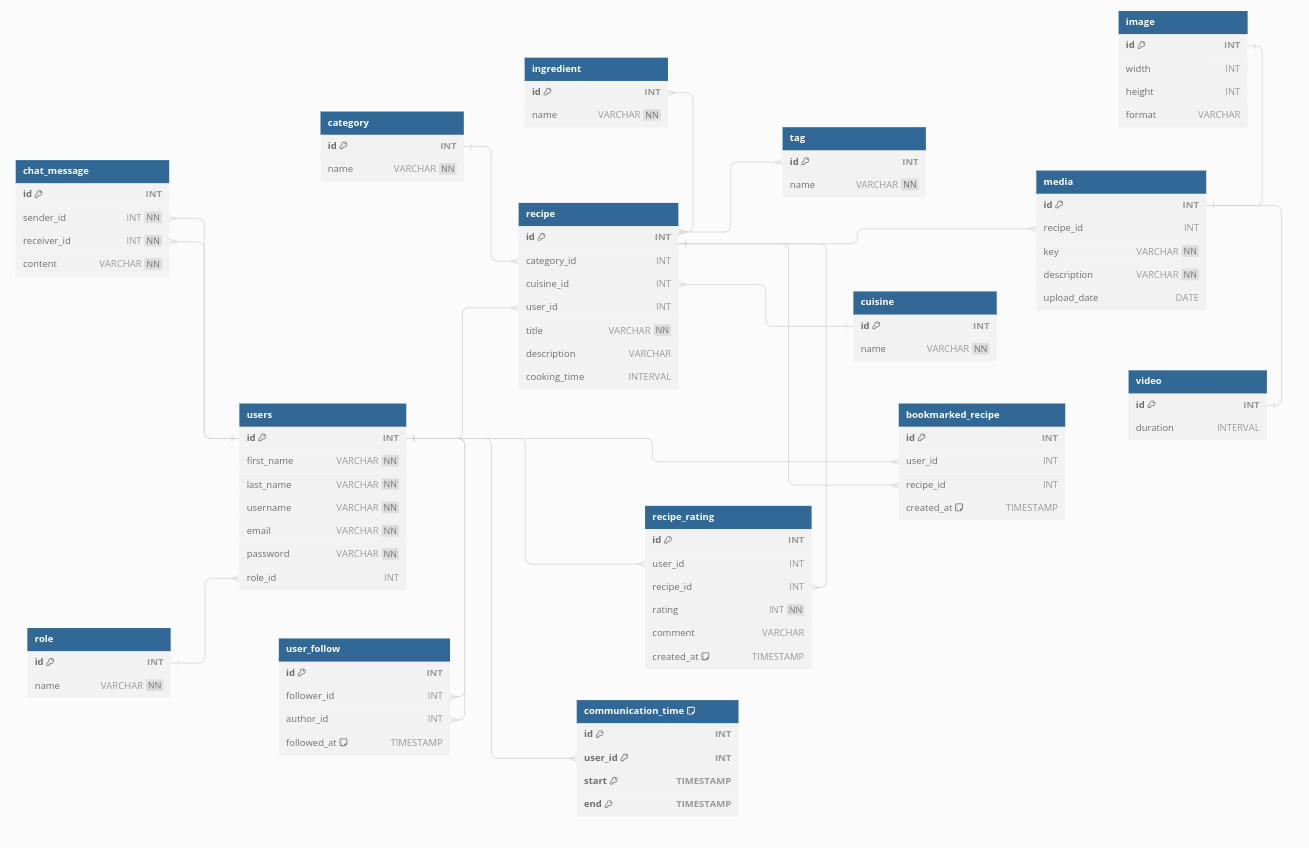
\includegraphics[scale=0.45]{dijagrami/dijagram_baze.png}} 
				\centering
				\caption{Dijagram baze podataka}
				\label{fig:bpdiag}
			\end{figure}
			
			
		\section{Dijagram razreda}

		Slike 4.2, 4.3 i 4.4 prikazuju razrede koji pripadaju backend dijelu odabrane
		arhitektura sustava (MVC). Razredi prikazani na slici 4.3 nasljeđuju Controller
		razred. Metode unutar tih razreda služe za manipulaciju podatcima pomoću
		DTO-a (Data Transfer Object). Podatci se dobivaju kroz metode koje su implementirane
		u Model razredima. Metode unutar Controller razreda odgovorne su za generiranje JSON datoteka
		i odgovarajućeg HTML statusnog koda kao povratne informacije na njihovo izvršavanje.

		\eject
		
		\begin{figure}[H]
			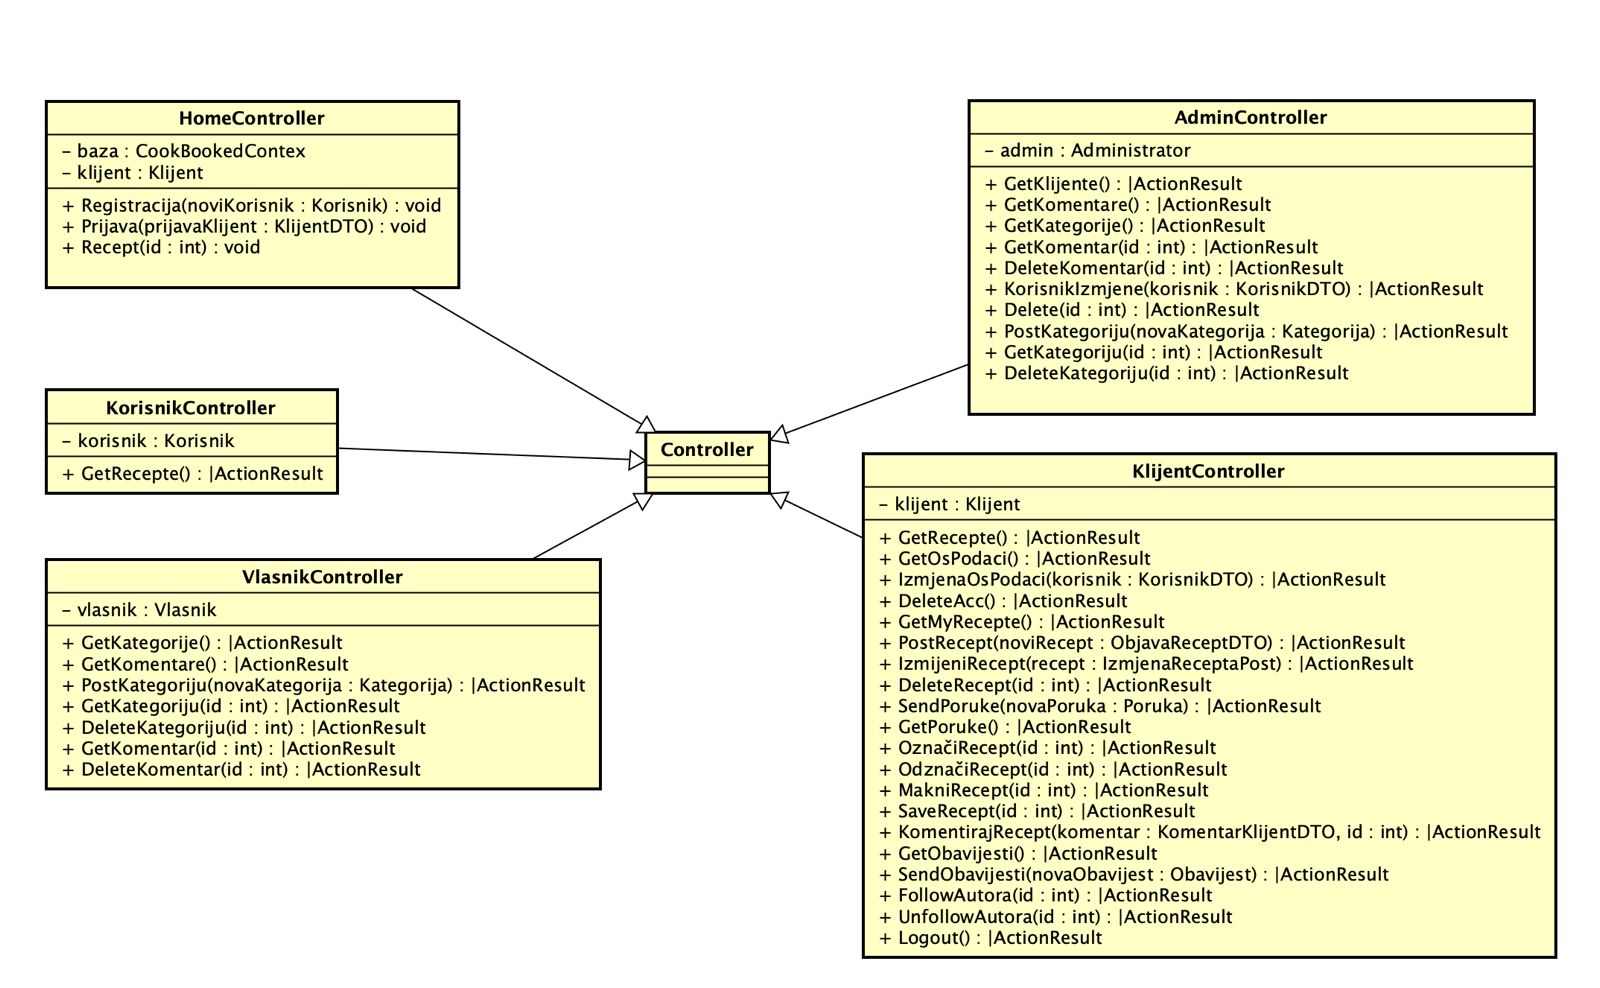
\includegraphics[scale=0.32]{dijagrami/razdijag_controller.jpeg} 
			\centering
			\caption{Dijagram razreda - dio Controllers}
			\label{fig:bpdiag}
		\end{figure}

		\eject

		\begin{figure}[H]
			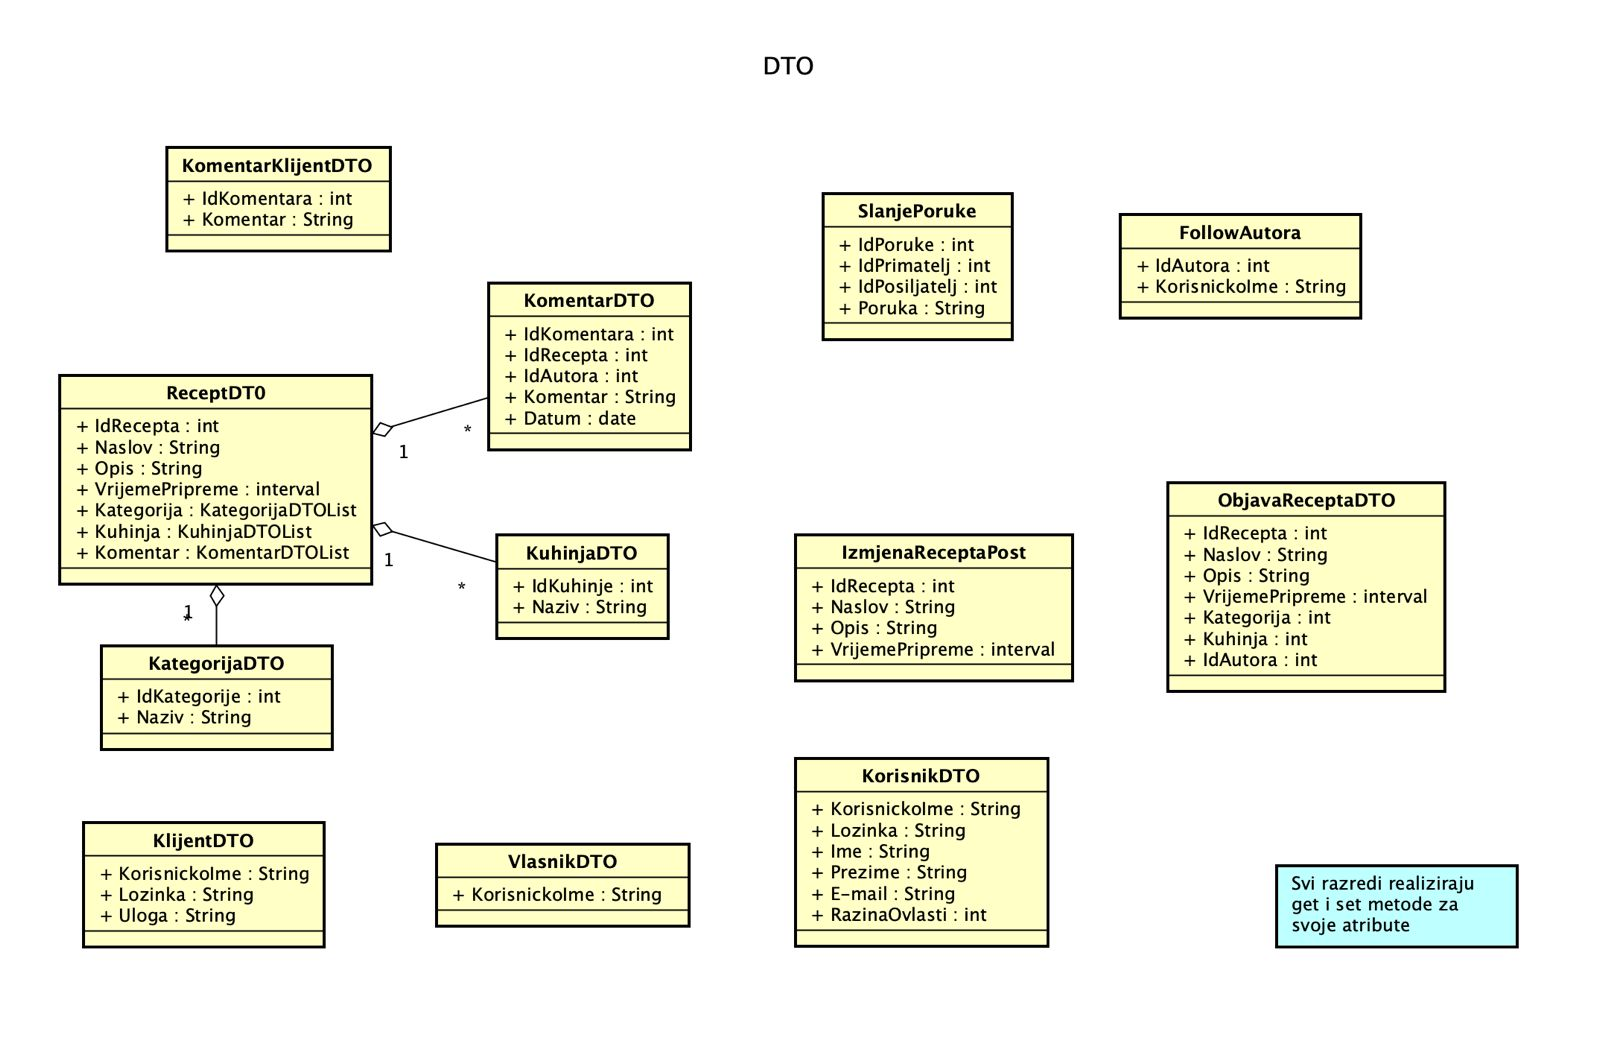
\includegraphics[scale=0.32]{dijagrami/razdijag_dto.jpeg}
			\centering
			\caption{Dijagram razreda - dio Data transfer objects}
			\label{fig:bpdiag}
		\end{figure}

		\eject

		\begin{figure}[H]
			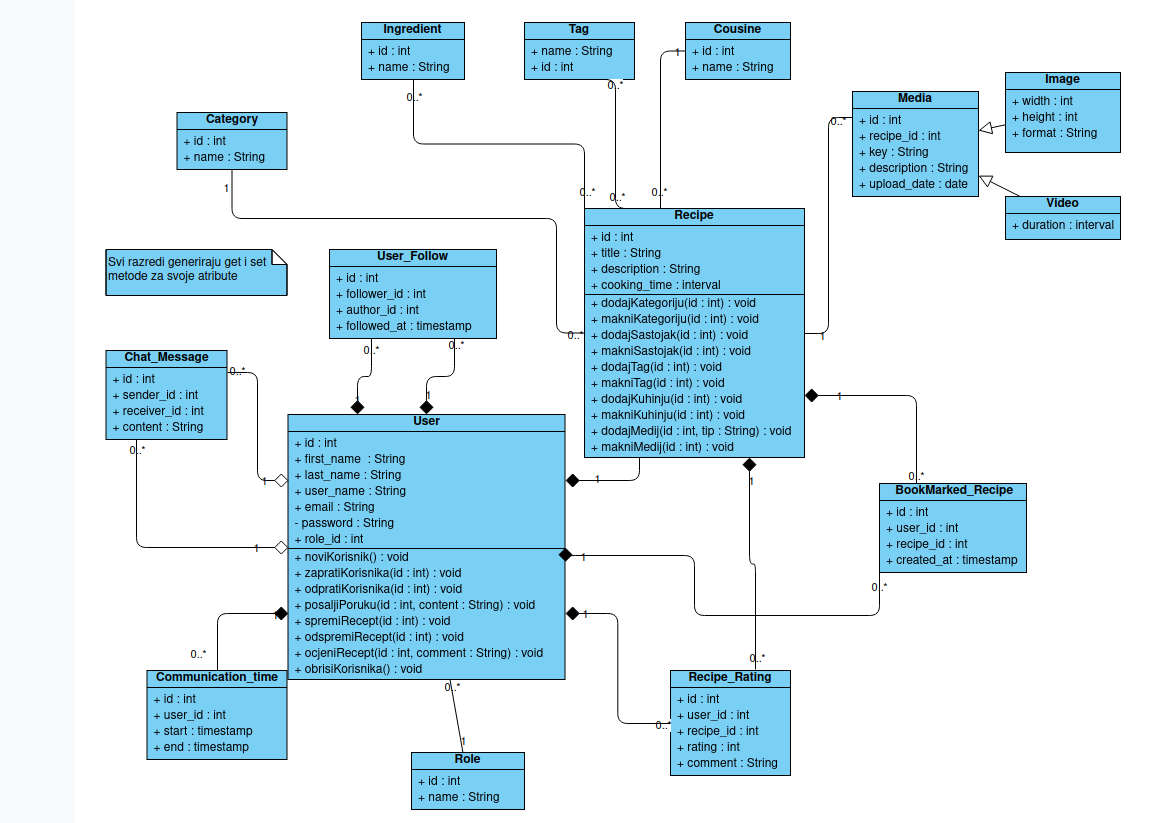
\includegraphics[scale=0.4]{dijagrami/razdijag_model.png}
			\centering
			\caption{Dijagram razreda - dio Models}
			\label{fig:bpdiag}
		\end{figure}

		\eject

		\section{Dijagram stanja}
		Dijagram stanja prikazuje stanja objekata te prijelaze iz jednog stanja u drugo
		temeljene na događajima. Na slici 4.5 prikazan je dijagram stanja za registriranog
		korisnika.

		\noindent Nakon što se prijavi, klijent je preusmjeren na početnu stranicu s koje može
		pristupiti ostalim stranicama ("Postavke profila", "Moji recepti", "Dodavanje recepta", "Stranica s receptima",
		"Pregledavanje pristiglih poruka").

		\noindent Ako klijent odluči pregledavati recepte, iz padajućeg izbornika ima opciju
		filtrirati iste po kategoriji, kuhinji ili sastojcima recepta. Nakon prikaza svih filtriranih
		recepata, klijent može detaljnije pregledati svaki pojedinačni recept te objaviti komentar ili
		kontaktirati njegova autora.

		\noindent Preostale stranice nude očekivane opcije vezane uz postavke korisničkog profila,
		brisanje korisničkog profila, uređivanje već objavljenih recepata, njihovo brisanje, dodavanje novih
		te komunikaciju sa korisnicima koji sutemeljem već objavljenih recepata klijenta kontaktirali.

		\begin{figure}[H]
			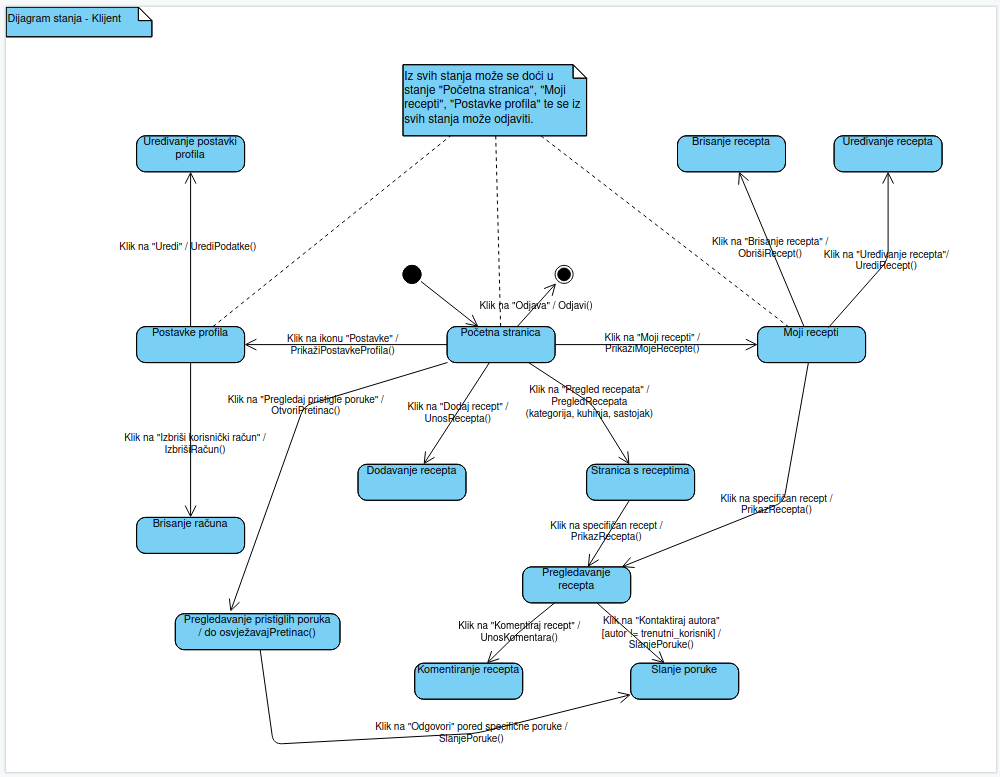
\includegraphics[scale=0.42]{dijagrami/dijagram_stanja.png}
			\centering
			\caption{Dijagram stanja}
			\label{fig:bpdiag}
		\end{figure}
		\eject
		
		\section{Dijagram aktivnosti}

		\noindent Na slici 4.6 prikazi su procesi akcija koje korisnik može izvršiti ukoliko se nađe na početnoj stranici.
		Detaljnije je obrađen slučaj ako korisnik želi pregledati pojedine recepte.
		Korisnik se prijavi u sustav, odabere koju stranicu želi vidjeti (detaljnije obrađena stranica prikaza recepata),
		a odabirom prikaza recepata prikažu mu se recepti. Odabirom pojedinog recepta korisnik može komentirati recept,
		poslati poruku autoru ili, ako je recept njegov, urediti podatke o receptu.

		\noindent Svaka od akcija uključuje ispunjenje određe forme od strane korisnika, slanje upita od strane web-aplikacije
		bazi podatakam potom odgovor baze podataka na taj upit te prikaz tog odgovora od strane web-aplikacije.

		\eject

		\begin{figure}[H]
			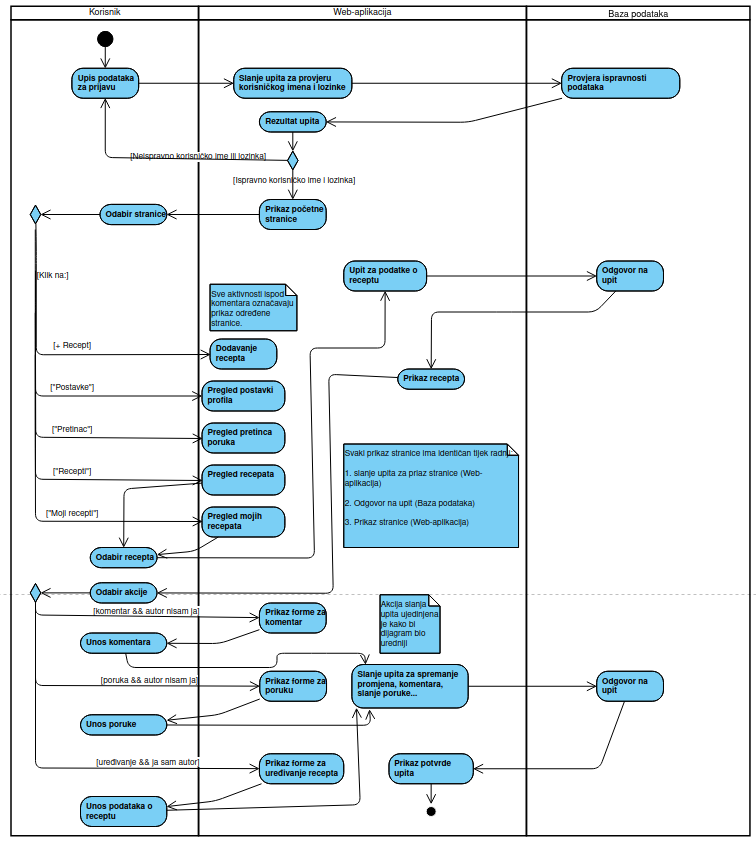
\includegraphics[scale=0.6]{dijagrami/dijagram_aktivnosti.png}
			\centering
			\caption{Dijagram aktivnosti}
			\label{fig:bpdiag}
		\end{figure}
		\eject
	%\chapter{Implementacija i korisničko sučelje}
		
		
		\section{Korištene tehnologije i alati}
		
			Komunikacija u timu realizirana je korištenjem aplikacije Discord\footnote[1]{https://discord.com/} te aplikacija WhatsApp\footnote[2]{https://www.whatsapp.com/}. Za izradu UML dijagrama korišten je
			web servis Visual Paradigm Online\footnote[3]{https://online.visual-paradigm.com/}, a kao sustav za upravljanje izvornim kodom Git\footnote[4]{https://git-scm.com/}. Udaljeni repozitorij projekta je dostupan na
			web platformi GitHub\footnote[5]{https://github.com/}.
			\smallbreak
			\noindent Kao razvojna okruženja korišteni su:
			\begin{itemize}
				\item IntelliJ IDEA Ultimate\footnote[6]{https://online.visual-paradigm.com/} - \textit{\textbf{backend}}
				\item Microsoft Visual Studio\footnote[7]{https://visualstudio.microsoft.com/} - \textit{\textbf{frontend, dokumentacija}}
			\end{itemize}
			\noindent Integrirana razvojna okruženja tvrtke JetBrains (1.), tj. Microsoft (2.).
			\smallbreak
			Aplikacija je napisana koristeći radni okvir Spring Boot\footnote[8]{https://spring.io/projects/spring-boot/} i jezik Java\footnote[9]{https://www.java.com/en/} za izradu 
			\textit{backend-a}, tj. radni okvir React\footnote[10]{https://reactjs.org/} i jezik JavaScript\footnote[11]{https://www.javascript.com/} za izradu \textit{frontend-a}.
			\smallbreak
			Baza podataka nalazi se na poslužitelju u oblaku DigitalOcean\footnote[12]{https://www.digitalocean.com/}.
			\eject 
		
	
		\section{Ispitivanje programskog rješenja}
			
			\textbf{\textit{dio 2. revizije}}\\
			
			 \textit{U ovom poglavlju je potrebno opisati provedbu ispitivanja implementiranih funkcionalnosti na razini komponenti i na razini cijelog sustava s prikazom odabranih ispitnih slučajeva. Studenti trebaju ispitati temeljnu funkcionalnost i rubne uvjete.}
	
			
			\subsection{Ispitivanje komponenti}
			\textit{Potrebno je provesti ispitivanje jedinica (engl. unit testing) nad razredima koji implementiraju temeljne funkcionalnosti. Razraditi \textbf{minimalno 6 ispitnih slučajeva} u kojima će se ispitati redovni slučajevi, rubni uvjeti te izazivanje pogreške (engl. exception throwing). Poželjno je stvoriti i ispitni slučaj koji koristi funkcionalnosti koje nisu implementirane. Potrebno je priložiti izvorni kôd svih ispitnih slučajeva te prikaz rezultata izvođenja ispita u razvojnom okruženju (prolaz/pad ispita). }
			
			
			
			\subsection{Ispitivanje sustava}
			
			 \textit{Potrebno je provesti i opisati ispitivanje sustava koristeći radni okvir Selenium\footnote{\url{https://www.seleniumhq.org/}}. Razraditi \textbf{minimalno 4 ispitna slučaja} u kojima će se ispitati redovni slučajevi, rubni uvjeti te poziv funkcionalnosti koja nije implementirana/izaziva pogrešku kako bi se vidjelo na koji način sustav reagira kada nešto nije u potpunosti ostvareno. Ispitni slučaj se treba sastojati od ulaza (npr. korisničko ime i lozinka), očekivanog izlaza ili rezultata, koraka ispitivanja i dobivenog izlaza ili rezultata.\\ }
			 
			 \textit{Izradu ispitnih slučajeva pomoću radnog okvira Selenium moguće je provesti pomoću jednog od sljedeća dva alata:}
			 \begin{itemize}
			 	\item \textit{dodatak za preglednik \textbf{Selenium IDE} - snimanje korisnikovih akcija radi automatskog ponavljanja ispita	}
			 	\item \textit{\textbf{Selenium WebDriver} - podrška za pisanje ispita u jezicima Java, C\#, PHP koristeći posebno programsko sučelje.}
			 \end{itemize}
		 	\textit{Detalji o korištenju alata Selenium bit će prikazani na posebnom predavanju tijekom semestra.}
			
			\eject 
		
		
		\section{Dijagram razmještaja}
			
			\textbf{\textit{dio 2. revizije}}
			
			 \textit{Potrebno je umetnuti \textbf{specifikacijski} dijagram razmještaja i opisati ga. Moguće je umjesto specifikacijskog dijagrama razmještaja umetnuti dijagram razmještaja instanci, pod uvjetom da taj dijagram bolje opisuje neki važniji dio sustava.}
			
			\eject 
		
		\section{Upute za puštanje u pogon}
		
			\textbf{\textit{dio 2. revizije}}\\
		
			 \textit{U ovom poglavlju potrebno je dati upute za puštanje u pogon (engl. deployment) ostvarene aplikacije. Na primjer, za web aplikacije, opisati postupak kojim se od izvornog kôda dolazi do potpuno postavljene baze podataka i poslužitelja koji odgovara na upite korisnika. Za mobilnu aplikaciju, postupak kojim se aplikacija izgradi, te postavi na neku od trgovina. Za stolnu (engl. desktop) aplikaciju, postupak kojim se aplikacija instalira na računalo. Ukoliko mobilne i stolne aplikacije komuniciraju s poslužiteljem i/ili bazom podataka, opisati i postupak njihovog postavljanja. Pri izradi uputa preporučuje se \textbf{naglasiti korake instalacije uporabom natuknica} te koristiti što je više moguće \textbf{slike ekrana} (engl. screenshots) kako bi upute bile jasne i jednostavne za slijediti.}
			
			
			 \textit{Dovršenu aplikaciju potrebno je pokrenuti na javno dostupnom poslužitelju. Studentima se preporuča korištenje neke od sljedećih besplatnih usluga: \href{https://aws.amazon.com/}{Amazon AWS}, \href{https://azure.microsoft.com/en-us/}{Microsoft Azure} ili \href{https://www.heroku.com/}{Heroku}. Mobilne aplikacije trebaju biti objavljene na F-Droid, Google Play ili Amazon App trgovini.}
			
			
			\eject 
	%\chapter{Zaključak i budući rad}
		
		\textbf{\textit{dio 2. revizije}}\\
		
		 \textit{U ovom poglavlju potrebno je napisati osvrt na vrijeme izrade projektnog zadatka, koji su tehnički izazovi prepoznati, jesu li riješeni ili kako bi mogli biti riješeni, koja su znanja stečena pri izradi projekta, koja bi znanja bila posebno potrebna za brže i kvalitetnije ostvarenje projekta i koje bi bile perspektive za nastavak rada u projektnoj grupi.}
		
		 \textit{Potrebno je točno popisati funkcionalnosti koje nisu implementirane u ostvarenoj aplikaciji.}
		
		\eject 
	\chapter*{Popis literature}
		\addcontentsline{toc}{chapter}{Popis literature}
	 	
 		\textbf{\textit{Kontinuirano osvježavanje}}
	
		\textit{Popisati sve reference i literaturu koja je pomogla pri ostvarivanju projekta.}
		
		
		\begin{enumerate}
			
			
			\item  Programsko inženjerstvo, FER ZEMRIS, \url{http://www.fer.hr/predmet/proinz}
			
			\item  I. Sommerville, "Software engineering", 8th ed, Addison Wesley, 2007.
			
			\item  T.C.Lethbridge, R.Langaniere, "Object-Oriented Software Engineering", 2nd ed. McGraw-Hill, 2005.
			
			\item  I. Marsic, Software engineering book``, Department of Electrical and Computer Engineering, Rutgers University, \url{http://www.ece.rutgers.edu/~marsic/books/SE}
			
			\item  The Unified Modeling Language, \url{https://www.uml-diagrams.org/}
			
			\item  Astah Community, \url{http://astah.net/editions/uml-new}
		\end{enumerate}
		
		 
	
	
	\begingroup
	\renewcommand*\listfigurename{Indeks slika i dijagrama}
	%\renewcommand*\listtablename{Indeks tablica}
	%\let\clearpage\relax
	\listoffigures
	%\vspace{10mm}
	%\listoftables
	\endgroup
	\addcontentsline{toc}{chapter}{Indeks slika i dijagrama}


	
	\eject 
		
	\chapter*{Dodatak: Prikaz aktivnosti grupe}
		\addcontentsline{toc}{chapter}{Dodatak: Prikaz aktivnosti grupe}
		
		\section*{Dnevnik sastajanja}
		
		\textbf{\textit{Kontinuirano osvježavanje}}\\
		
		\begin{packed_enum}

			\item  komunikacija - svakodnevna putem WhatsApp grupe
			\item[] \begin{packed_item}
				\item Datum: svakodnevno
				\item Prisustvovali: M. Dananić, P. Habjanec, D. Huić, V. Ivanić, L. Iveković, D. Ožvald, M. A. Stuhne
				\item Teme sastanka:
				\begin{packed_item}
					\item  napredak u područjima koda i dokumentacije
				\end{packed_item}
			\end{packed_item}

			\item  sastanak
			\item[] \begin{packed_item}
				\item Datum: 23.10.2023.
				\item Prisustvovali: M. Dananić, P. Habjanec, D. Huić, V. Ivanić, L. Iveković, D. Ožvald, M. A. Stuhne
				\item Teme sastanka:
				\begin{packed_item}
					\item  raspodjela posla
					\item  korištene tehnologije
					\item  initial commit
				\end{packed_item}
			\end{packed_item}
			
			\item  sastanak
			\item[] \begin{packed_item}
				\item Datum: 29.10.2023.
				\item Prisustvovali: M. Dananić, P. Habjanec, D. Huić, V. Ivanić, L. Iveković, D. Ožvald, M. A. Stuhne
				\item Teme sastanka:
				\begin{packed_item}
					\item  bitni zadatci do 2.11.2023.
					\item  dogovor oko dokumentacije
				\end{packed_item}
			\end{packed_item}
			
			%
			
		\end{packed_enum}
		
		\eject
		\section*{Tablica aktivnosti}
		
			\textbf{\textit{Kontinuirano osvježavanje}}\\
			
			 \textit{Napomena: Doprinose u aktivnostima treba navesti u satima po članovima grupe po aktivnosti.}

			\begin{longtblr}[
					label=none,
				]{
					vlines,hlines,
					width = \textwidth,
					colspec={X[7, l]X[1, c]X[1, c]X[1, c]X[1, c]X[1, c]X[1, c]X[1, c]}, 
					vline{1} = {1}{text=\clap{}},
					hline{1} = {1}{text=\clap{}},
					rowhead = 1,
				} 
			
				\SetCell[c=1]{c}{} & \SetCell[c=1]{c}{\rotatebox{90}{\textbf{Ime Prezime voditelja}}} & \SetCell[c=1]{c}{\rotatebox{90}{\textbf{Ime Prezime }}} &	\SetCell[c=1]{c}{\rotatebox{90}{\textbf{Ime Prezime }}} & \SetCell[c=1]{c}{\rotatebox{90}{\textbf{Ime Prezime }}} &	\SetCell[c=1]{c}{\rotatebox{90}{\textbf{Ime Prezime }}} & \SetCell[c=1]{c}{\rotatebox{90}{\textbf{Ime Prezime }}} &	\SetCell[c=1]{c}{\rotatebox{90}{\textbf{Ime Prezime }}} \\  
				Upravljanje projektom 		&  &  &  &  &  &  & \\ 
				Opis projektnog zadatka 	&  &  &  &  &  &  & \\ 
				
				Funkcionalni zahtjevi       &  &  &  &  &  &  &  \\ 
				Opis pojedinih obrazaca 	&  &  &  &  &  &  &  \\ 
				Dijagram obrazaca 			&  &  &  &  &  &  &  \\ 
				Sekvencijski dijagrami 		&  &  &  &  &  &  &  \\ 
				Opis ostalih zahtjeva 		&  &  &  &  &  &  &  \\ 

				Arhitektura i dizajn sustava	 &  &  &  &  &  &  &  \\ 
				Baza podataka				&  &  &  &  &  &  &   \\ 
				Dijagram razreda 			&  &  &  &  &  &  &   \\ 
				Dijagram stanja				&  &  &  &  &  &  &  \\ 
				Dijagram aktivnosti 		&  &  &  &  &  &  &  \\ 
				Dijagram komponenti			&  &  &  &  &  &  &  \\ 
				Korištene tehnologije i alati 		&  &  &  &  &  &  &  \\ 
				Ispitivanje programskog rješenja 	&  &  &  &  &  &  &  \\ 
				Dijagram razmještaja			&  &  &  &  &  &  &  \\ 
				Upute za puštanje u pogon 		&  &  &  &  &  &  &  \\  
				Dnevnik sastajanja 			&  &  &  &  &  &  &  \\ 
				Zaključak i budući rad 		&  &  &  &  &  &  &  \\  
				Popis literature 			&  &  &  &  &  &  &  \\  
				&  &  &  &  &  &  &  \\ \hline 
				\textit{Dodatne stavke kako ste podijelili izradu aplikacije} 			&  &  &  &  &  &  &  \\ 
				\textit{npr. izrada početne stranice} 				&  &  &  &  &  &  &  \\  
				\textit{izrada baze podataka} 		 			&  &  &  &  &  &  & \\  
				\textit{spajanje s bazom podataka} 							&  &  &  &  &  &  &  \\ 
				\textit{back end} 							&  &  &  &  &  &  &  \\  
				 							&  &  &  &  &  &  &\\ 
			\end{longtblr}
					
					
		\eject


\end{document} %naredbe i tekst nakon ove naredbe ne ulaze u izgrađen dokument 


